\documentclass[10pt]{beamer}
\useoutertheme{metropolis}
\useinnertheme{metropolis}
\usefonttheme{metropolis}
\usecolortheme{metropolis} % more at http://www.deic.uab.es/~iblanes/beamer_gallery/index_by_color.html

% -----------------------------------------------------------------------------
% Title and Author Information -- Need to Edit
% -----------------------------------------------------------------------------

\title{Introduction to Neural Nets}
\subtitle{Columbia Water Center Neural Network Working Group}
\date{\today}
\author{James Doss-Gollin \and Tristan Eisenhart}
\institute{Columbia University}

% -----------------------------------------------------------------------------
% Package Configuration -- Don't Necessarily Need to Edit
% -----------------------------------------------------------------------------

% Packages with Options
\usepackage[english]{babel}

% Package List
\usepackage{
	siunitx, % for SI notation
	wrapfig, % for figures with text next to them
	booktabs, % for better (alternative?) tables
  csquotes, % better biblatex
	cleveref, % better citations
	physics, % for better notation
	array, % for table stuff
}

% figures
\usepackage{graphicx}
\graphicspath{{fig/}} % can add more

% macros
\usepackage{xspace}
\newcommand*{\eg}{e.g.\@\xspace}
\newcommand*{\ie}{i.e.\@\xspace}
% cont'd
\makeatletter
\newcommand*{\etc}{%
    \@ifnextchar{.}%
        {etc}%
        {etc.\@\xspace}%
}
\makeatother

% Biblatex Setup using a file called library.bib
\usepackage[
  backend=biber,
  doi=true,
  url=false,
  isbn=false,
  %style=authoryear-comp,
  style=numeric-comp,
  natbib=true,
  backref=false,
  maxbibnames=2,
  %mincitenames=2,
  maxcitenames=2,
  uniquename=false,
  uniquelist=false
  ]{biblatex}
\renewcommand{\refname}{References}
\renewbibmacro{in:}{}
\AtEveryBibitem{\clearfield{month}\clearfield{pages}}
\addbibresource{library.bib} % even better to symlink
\setbeamertemplate{bibliography item}[text] % don't print the symbols

% -----------------------------------------------------------------------------
% BEGIN DOCUMENT HERE
% -----------------------------------------------------------------------------

\begin{document}

% TITLE PAGE
\maketitle

\begin{frame}{Table of contents}
  \setbeamertemplate{section in toc}[sections numbered]
  \tableofcontents[hideallsubsections]
\end{frame}

% -----------------------------------------------------------------------------
% WHAT CAN DEEP LEARNING DO?
% -----------------------------------------------------------------------------

\begin{frame}
	\frametitle{Disclaimer}
	\begin{itemize}
		\item I am not an expert in deep learning and none of the following content is original.
		Mostly it is poached from lecture notes by Peter Belhumeur for his \href{www.deeplearningforcomputervision.com/}{deep learning for computer vision} class, but there is also content taken from \citet{Friedman2001,James2013,Goodfellow-et-al-2016}.
		\item I highly recommend checking out the above sources
		\item This is not intended to be distributed outside the Columbia Water Center.
	\end{itemize}
\end{frame}

\section{What Can Deep Learning Do?}

\begin{frame}
	\frametitle{What Is Machine Learning}
	Difficult to define!
	\begin{itemize}
		\item Vocab: machine learning, statistics, quantitative modeling, deep learning
		\item ML: more focus on making out-of-sample predictions which minimize some loss function
		\item ML: In general less focus on inference
		\item Scale to large data sets (large $N$) and high dimensions (large $p$)
		\item Deep learning is state-of-art ML algorithm for some types of problem
	\end{itemize}
\end{frame}

\begin{frame}
	\frametitle{Some Cool Demos}
	\begin{itemize}
		\item \href{https://blogs.dropbox.com/tech/2016/08/fast-and-accurate-document-detection-for-scanning/}{Dropbox Document Detection}
		\item \href{http://www.cs.toronto.edu/~graves/handwriting.cgi?text=I+am+really+hungry&style=&bias=0.15&samples=3}{Text to handwriting}
		\item \href{https://www.clarifai.com/demo}{Image Classification/Captioning}
		\item \href{http://www.birdsnap.com/species/}{Bird Identification}
	\end{itemize}
\end{frame}

% -----------------------------------------------------------------------------
% MACHINE LEARNING
% -----------------------------------------------------------------------------

\section{All About Classifiers}

\begin{frame}
	\frametitle{Linear Regression}
	We've all seen linear regression: predict value $y$ given data $\vb{x}$ with
	\begin{equation}
		\hat{y} = \vb{\theta}^T \vb{x}
	\end{equation}
	Note the notation: $\theta$ typically used to refer to parameters. $\vb{x}$ includes column of 1's for the intercept.
	\begin{figure}
		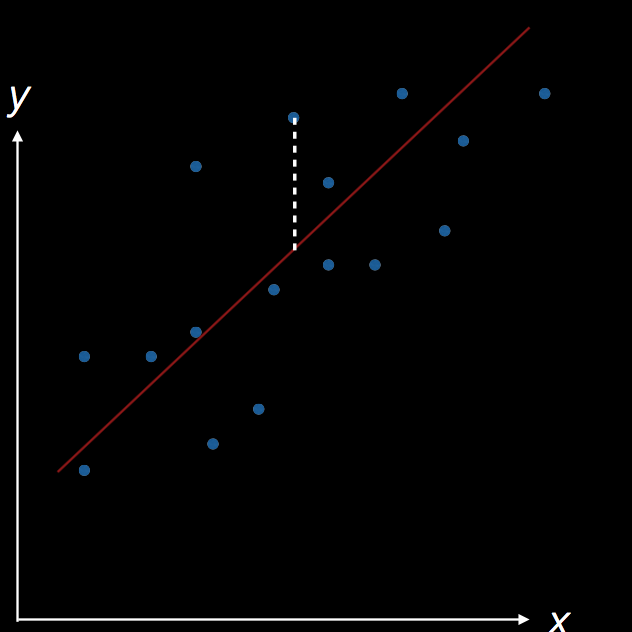
\includegraphics[width=\textwidth,height=0.3\textheight,keepaspectratio=true]{linear_regression.png}
		\caption{Linear Regression}
		\label{fig:linear-regression}
	\end{figure}
\end{frame}

\begin{frame}
	\frametitle{Classification}
	Take data and predict $1+$ categories
	\begin{figure}
		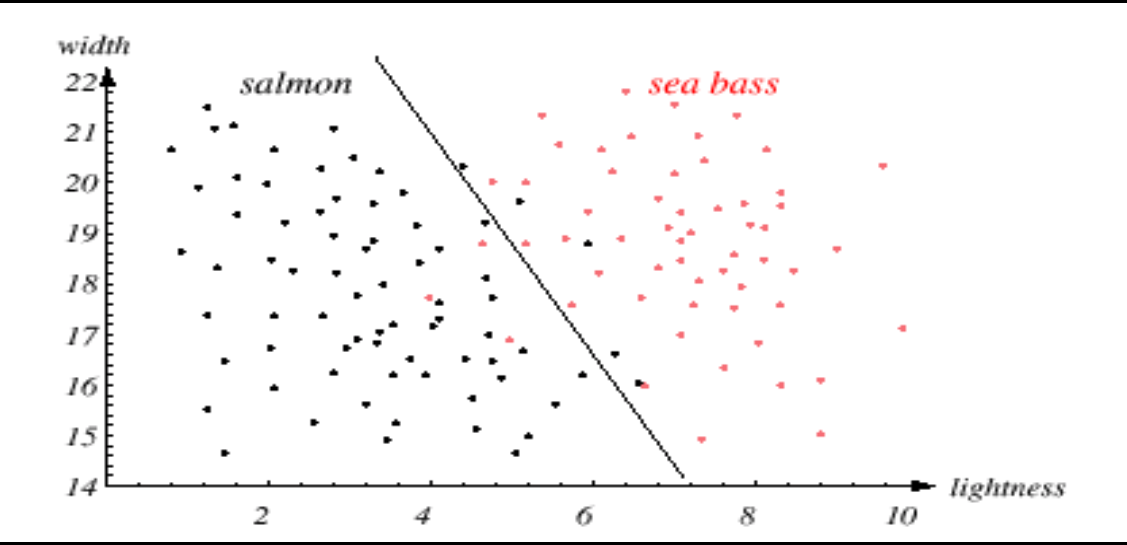
\includegraphics[width=\textwidth,height=0.6\textheight,keepaspectratio=true]{fish_scatter.png}
		\caption{A Scatter Plot}
		\label{fig:fish-scatter}
	\end{figure}
\end{frame}

\begin{frame}
	\frametitle{Conditional Probability}
	\begin{equation}
		p \qty(A \big| B) = \frac{P \qty(A, B)}{P(B)} =\frac{P \qty(A) P \qty(B \big| A)}{P(B)}
	\end{equation}
	\begin{figure}
		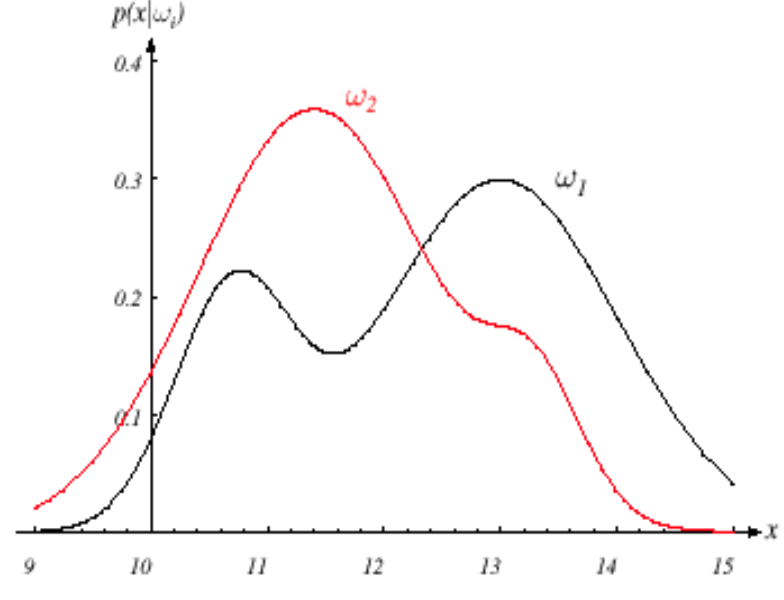
\includegraphics[width=0.5\textwidth,height=0.6\textheight,keepaspectratio=true]{pdf_fish.png}~
		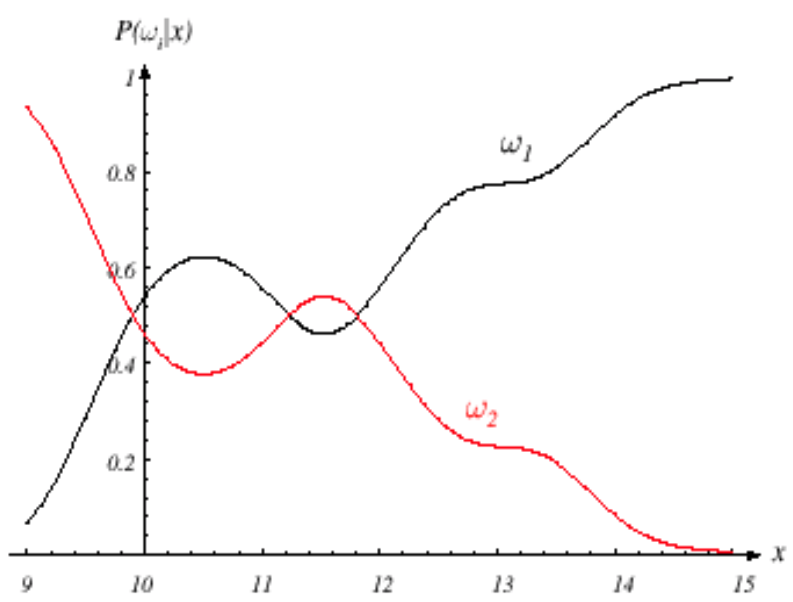
\includegraphics[width=0.5\textwidth,height=0.6\textheight,keepaspectratio=true]{posterior_fish.png}
		\caption{A naive fish classifier: (L) PDF (R) Posterior}
		\label{fig:pdf-fish}
	\end{figure}
\end{frame}

\begin{frame}
	\frametitle{Mathematical Framing}
	Let's think of a classifier as set of scalar functions $g_i(\vb{x})$ — one for each class $i$ — that assigns a score to the vector of feature values $\vb{x}$ and then choses the class $i$ with the highest score.
	In other words:
	\begin{exampleblock}{Choose class $i$ if}
		\begin{equation}
			g_i(\vb{x}) > g_j(\vb{x}) \forall j, i \neq j
		\end{equation}
	\end{exampleblock}
	This requires a good estimate of
	\[P \qty(\omega_i \big| \vb{x})\]
\end{frame}

\begin{frame}
	\frametitle{Curse of Dimensionality}
	\begin{itemize}
		\item If we have 3 dimensional feature space $\vb{x} \in \qty[0, 1]^3$
		\item We have 10000 training samples
		\item If we try to estimate our probability using a 3D histogram with 100 bins in each direction
		\item Each bin has (on average) 0.01 samples!
	\end{itemize}
	Thus we never have enough samples to sample high-dimensional feature space; \alert{Focus on finding decision surface which separates categories}
\end{frame}

\begin{frame}
	\frametitle{Many Possible Classifiers}
	With a classifier, what is our goal?
	\begin{figure}
		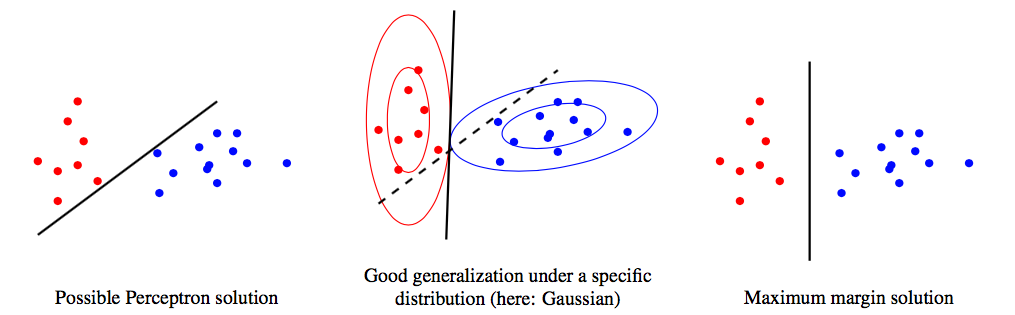
\includegraphics[width=\textwidth,height=\textheight,keepaspectratio=true]{classifier_possibilities.png}
		\caption{Maximum Margin tends to do well}
		\label{fig:maximum-margin}
	\end{figure}
	Support vector machine implements maximum-margin classifier -- skipping details for concision
\end{frame}

\begin{frame}
	\frametitle{Linear Classifier}
	Standard framing: training data $\qty(\vb{x}_i, y_i)$ with $i = 1, \ldots, N$ and $\vb{x}_i \in \mathbb{R}^d$ and $y_i \in \qty{-1, 1}$.
	Learn a linear classifier $f \qty( \vb{x}_i)$:
	\begin{equation}
		f \qty(\vb{x}_i) \begin{cases}\geq 0 & y = +1 \\ < 0 & y = -1\end{cases}
	\end{equation}
	and since we have a linear classifier, $f(\vb{x}) = \vb{\theta}^T \vb{x}$
\end{frame}

\begin{frame}
	\frametitle{Logistic (Sigmoid) Classifier}
	\begin{itemize}
		\item Extend linear classifier $f(\vb{x}) = \sigma^T \vb{x}$ to $\sigma \qty(f(\vb{x})) = \frac{1}{1 + e^{-f(x)}}$
		\item Predict $+1$ if $\sigma \geq 0.5$, $-1$ if $\sigma < 0.5$
	\end{itemize}
	\begin{figure}
		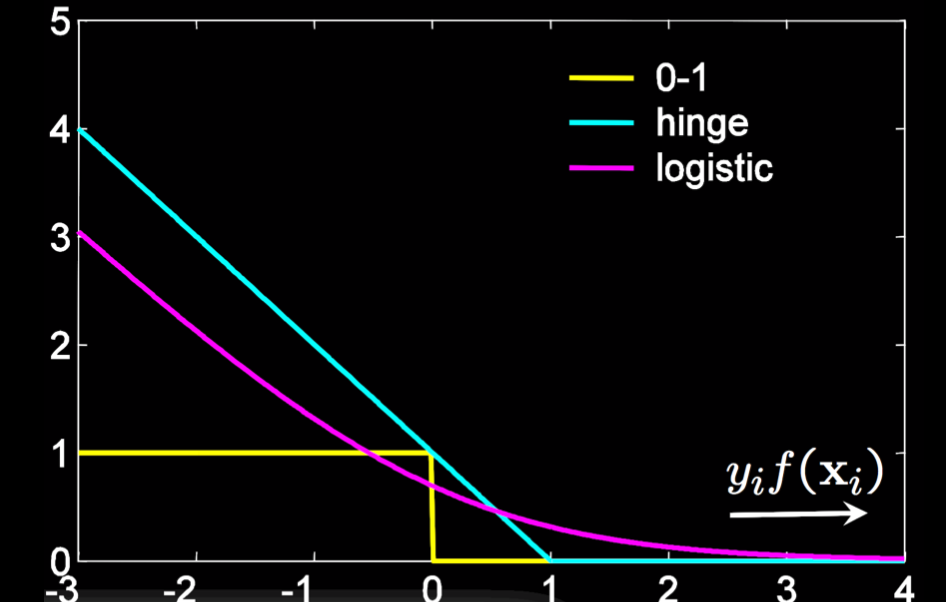
\includegraphics[width=\textwidth,height=0.45\textheight,keepaspectratio=true]{loss_fn.png}
		\caption{Comparison of loss functions}
		\label{fig:loss-function}
	\end{figure}
\end{frame}

\begin{frame}
	\frametitle{Maximum Likelihood Estimation}
	Maximizing the likelihood is the same as minimizing negative log-likelihood
	\begin{align}
		P \qty(y \big | \vb{x},\vb{\theta}) = \prod_{i=1}^N \frac{1}{1 + \exp \qty(-y_i f(\vb{x_i}))} \\
		L \qty(y \big | \vb{x},\vb{\theta}) = \sum_{i=1}^N \log \qty[1 + \exp \qty(-y_i f(\vb{x_i}))]
	\end{align}
\end{frame}

\begin{frame}
	\frametitle{Computational Graph}
	For this figure we have renamed $\theta$ to be $w$ and added a regularization term $\frac{\lambda}{2} \abs{\abs{\vb{\theta}}}^2$ to the cost function
	\begin{figure}
		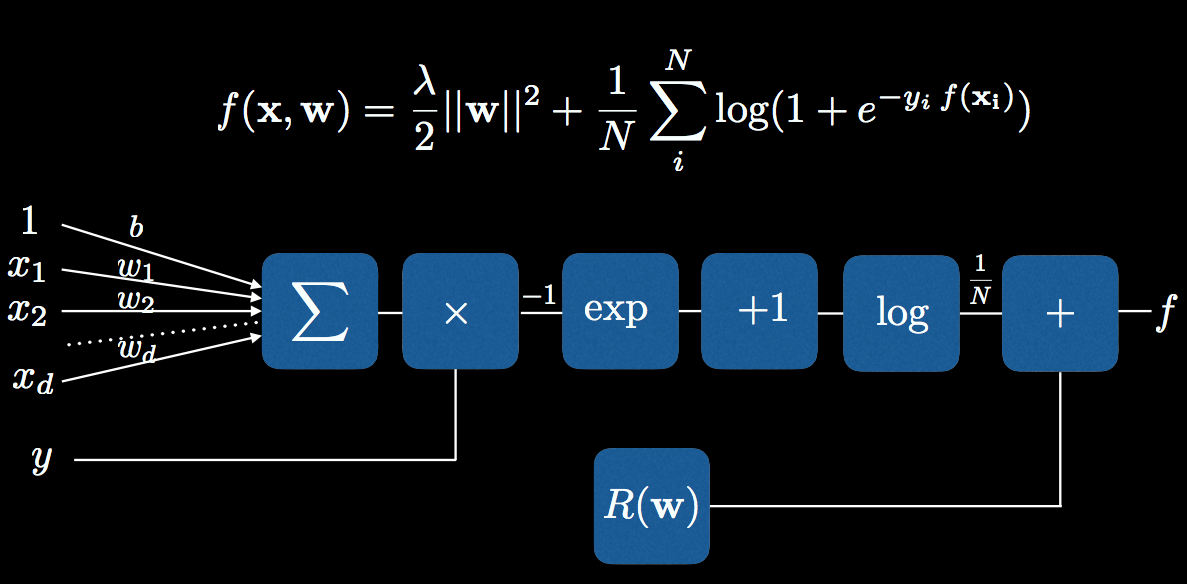
\includegraphics[width=\textwidth,height=0.5\textheight,keepaspectratio=true]{computational_graph.png}
		\caption{Computational graph for logistic regression}
		\label{fig:computational-graph}
	\end{figure}
\end{frame}

\begin{frame}
	\frametitle{Chain Rule}
	Given a training sample $\vb{x}$ let’s compute the gradient of $f$ with respect to the weights $\vb{\theta}$.
	\begin{figure}
		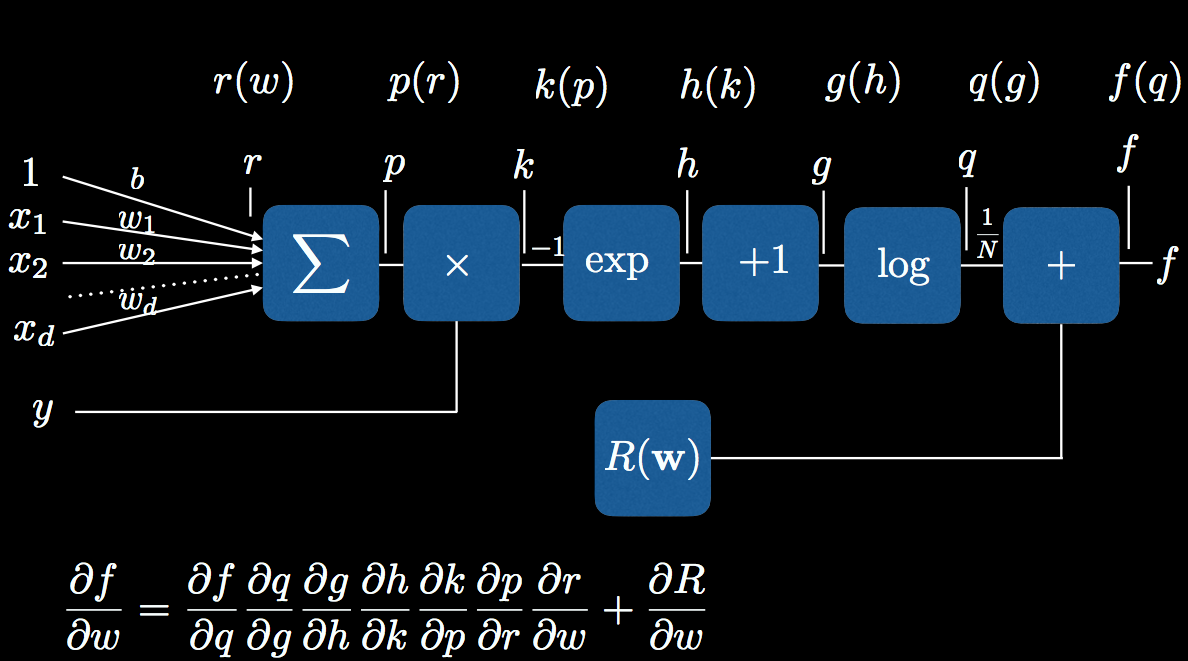
\includegraphics[width=\textwidth,height=0.5\textheight,keepaspectratio=true]{computational_derivatives.png}
		\caption{Chain rule for logistic regression example}
	\end{figure}
\end{frame}

\begin{frame}
	\frametitle{Gradient Descent}
	(There are more complicated ways to do this).
	Take our initial weights, choose a learning rate $\eta = 0.1$ say:
	\begin{equation}
		\vb{\theta}_{t+1} = \vb{\theta}_t - \eta \grad_{\vb{\theta}_t} f (\vb{\theta}_t)
	\end{equation}
\end{frame}

% -----------------------------------------------------------------------------
% BACK-PROPAGATION
% -----------------------------------------------------------------------------

\section{Neural Networks}

\begin{frame}
	\frametitle{Really?}
	James, are we going to show us some grainy pictures to illustrate the chain rule, and then claim we understand neural networks?
	\pause
	\vfill
	\alert{yep} (and not just because I'm writing this at midnight and want to sleep!)
\end{frame}

\begin{frame}
	\frametitle{Feedforward Network}
	We just need to generalize what we already learned.
	\begin{itemize}
		\item Let $y = f^*(\vb{x})$ be some function we don't know but want to approximate given data -- could be a classifier boundary!
		\item Try to learn parameters $\theta$ to approximate this
	\end{itemize}
	A feedforward network has \emph{no} feedback -- layers are composed of functions (``layers'') so that (\eg)
	\begin{equation}
		f (\vb{x}) = l^3(l^2(l^1(\vb{x})))
	\end{equation}
\end{frame}

\begin{frame}[standout]
  The network is thus mapping $\vb{x}$ to a feature space $\phi(\vb{x})$ in which (ideally...) the samples are linearly separable!
\end{frame}

\begin{frame}
	\frametitle{XOR 1}
	Let's see how this works.
	Take a problem where a linear classifier is useless:
	\begin{figure}
		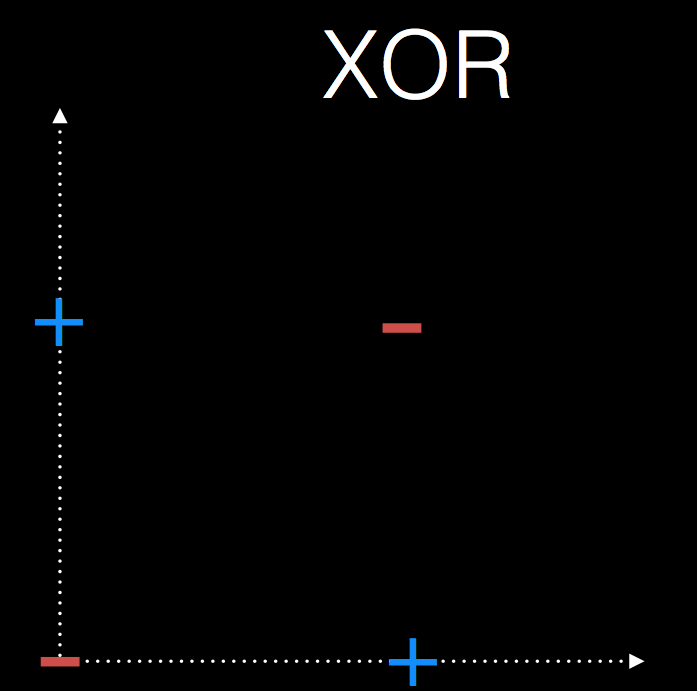
\includegraphics[width=\textwidth,height=0.5\textheight,keepaspectratio=true]{xor.png}
		\caption{The XOR Classification Problem}
	\end{figure}
\end{frame}

\begin{frame}
	\frametitle{XOR 2}
	Now let's add a single ``hidden'' layer:
	\begin{align}
		\vb{x} &\rightarrow^{w_1} \vb{h} \rightarrow^{w_2} y \\
		\pause
		h &= g(w_1^T \vb{x} + \vb{c}) \\
		y &= w_2^T \vb{h} + \vb{b} \\
		&= w_2^T g(w_1^T \vb{x} + \vb{v}) + b
	\end{align}
	\pause
	Now let's try setting $g(z) = \max(0, z)$ ``ReLU Function''
\end{frame}

\begin{frame}
	\frametitle{XOR 3}
	Now let's go back to the XOR problem!
	Let's let\\
		$w_1 = \qty[\begin{matrix}1&1\\1&1\end{matrix}]$, $\vb{c} = \qty[\begin{matrix}0\\-1\end{matrix}]$, $w_2 = \qty[\begin{matrix}1\\-2\end{matrix}]$, $b=0$
	and our samples\\
		$X=\qty[\begin{matrix}0&1&0&1\\0&0&1&1\end{matrix}]^T$
\end{frame}

\begin{frame}
	\frametitle{XOR 4}
	\begin{align}
		w_1^T \vb{x} + \vb{c} &= \qty[\begin{matrix}0&1&1&2\\-1&0&0&1\end{matrix}] \\
		h &= \max \qty(0, w_1^T \vb{x} + \vb{c}) \\
		&= \qty[\begin{matrix}0&1&1&2\\0&0&0&1\end{matrix}] \\
		y &= w_2^T h + b \\
		&= \qty[0 1 1 0]
	\end{align}
\end{frame}

\begin{frame}
	\frametitle{XOR Finally Done!}
	\begin{figure}
		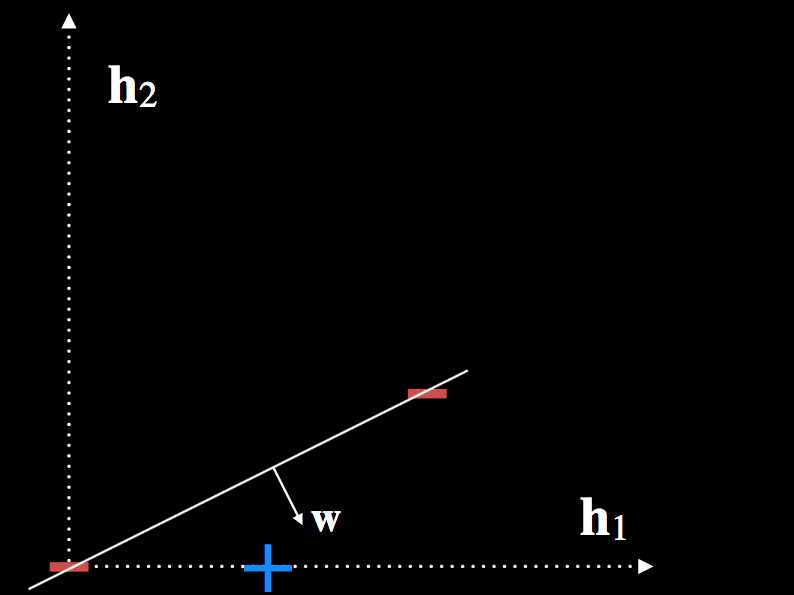
\includegraphics[width=\textwidth,height=0.75\textheight,keepaspectratio=true]{xor_mapped.png}
		\caption{So it worked! $h = \phi(\vb{x})$}
	\end{figure}
\end{frame}

\begin{frame}
	\frametitle{Training with Back-Propagation}
	\begin{enumerate}
		\item Create noisy XOR data
		\item Choose loss function for binary classifier (sigmoid is good -- or Softplus)
	\end{enumerate}
	\begin{figure}
		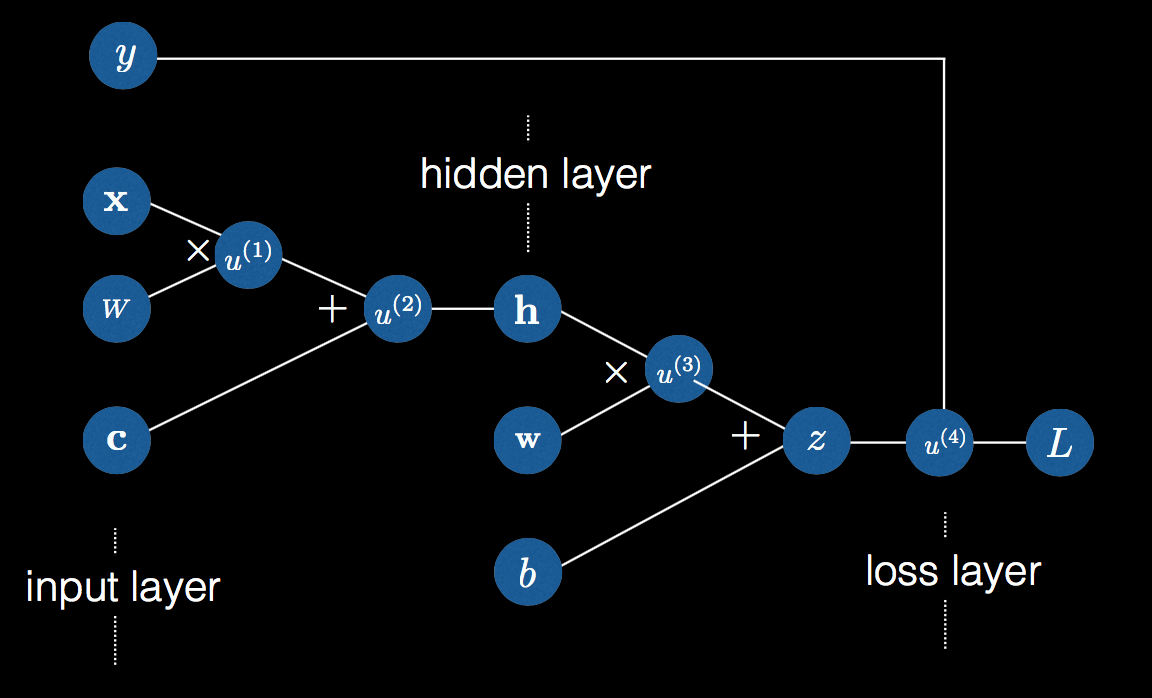
\includegraphics[width=\textwidth,height=0.55\textheight,keepaspectratio=true]{cgraph_hidden.png}
		\caption{Computational graph with a hidden layer}
	\end{figure}
\end{frame}

% -----------------------------------------------------------------------------
% CHALLENGES
% -----------------------------------------------------------------------------

\section{Challenges in Machine Learning}

\begin{frame}
	\frametitle{Over-fitting}
	\begin{figure}
		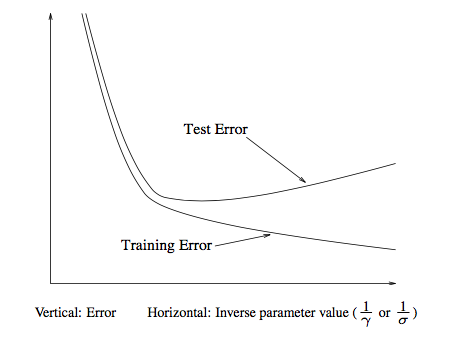
\includegraphics[width=\textwidth,height=0.85\textheight,keepaspectratio=true]{overfit_graph.png}
		\caption{Over-fitting can be a huge challenge!}
	\end{figure}
\end{frame}

\begin{frame}
	\frametitle{Over-fitting Example}
	\begin{figure}
		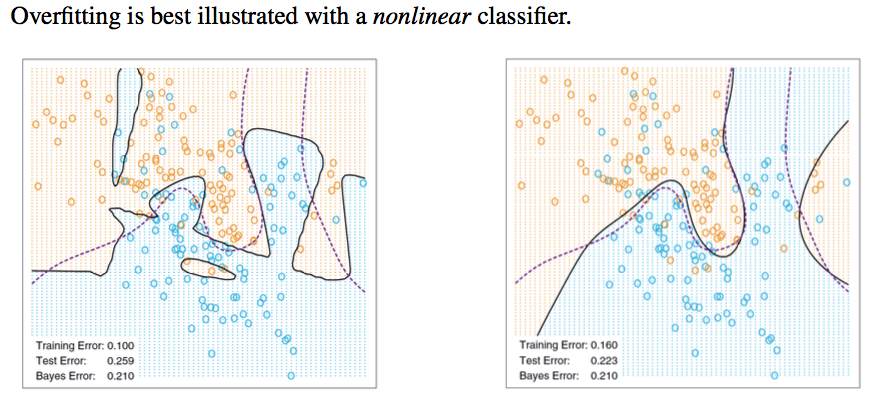
\includegraphics[width=\textwidth,height=0.85\textheight,keepaspectratio=true]{overfit_scatter.png}
		\caption{An example of overfit data}
	\end{figure}
\end{frame}
\begin{frame}
	\frametitle{Over-fitting Example2}
	\begin{figure}
		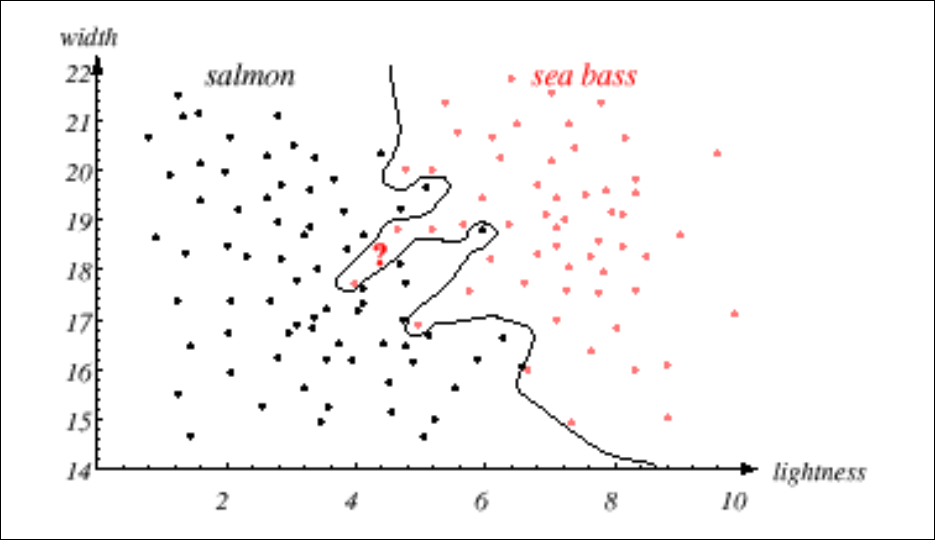
\includegraphics[width=\textwidth,height=0.85\textheight,keepaspectratio=true]{classifier_fish.png}
		\caption{Another example of overfit data}
	\end{figure}
\end{frame}

\begin{frame}
	\frametitle{Computer Vision}
	Also there are
	\begin{itemize}
		\item Geometric invariants for rigid transformations of 3-D objects viewed under perspective projective projection do not exist\citep{Burns:1993ih}
		\item Illumination invariants for 3D ojbects to not exist \citep{Chen:ba}
	\end{itemize}
\end{frame}

\begin{frame}
	\frametitle{Regularization}
	\begin{quotation}
		The goal of regularization is to prevent overfitting the training data with the hope that this improves generalization, \ie, the ability to correctly handle data that the network has not trained on.
	\end{quotation}
	\alert{Go to Peter Belhumeur's slides on regularization (begin p.365 of his course notes!)}
\end{frame}

% -----------------------------------------------------------------------------
% QUESTIONS, BIBLIOGRAPHY
% -----------------------------------------------------------------------------

\begin{frame}%[t,allowframebreaks]
	\frametitle{References}
	\renewcommand*{\bibfont}{\tiny}
	\printbibliography[heading=none]
\end{frame}

\begin{frame}
	\frametitle{Some More Resources}
	As you check tutorials, be aware that there are subtle differences between python 2 and python 3 (\ie \texttt{print}).
	There are big differences between different versions of \texttt{tensorflow}.
	Using a \href{https://uoa-eresearch.github.io/eresearch-cookbook/recipe/2014/11/20/conda/}{custom conda environment} is a great way to manage versions -- read on your own :).
	Some other useful resources:
	\begin{itemize}

		\item DLCV course slides will be posted to Slack
		\item \href{http://www.deeplearningforcomputervision.com}{DLCV course website}
		\item \href{https://www.tensorflow.org/tutorials/}{Tensorflow tutorial}
		\item \href{https://www.datacamp.com/community/tutorials/tensorflow-tutorial\#gs.tELsmK4}{TF tutorial by Karlijn Willems}
		\item \href{http://cs231n.github.io/}{Stamford Deep Learning Class CS231}
		\href{https://medium.com/@karpathy/yes-you-should-understand-backprop-e2f06eab496b}{Blog post: why understanding back-propagation matters}
	\end{itemize}
\end{frame}

%\plain{}{Supplemental Information}
\begin{frame}[standout]
  Thanks!
\end{frame}

\end{document}
